\documentclass[conference]{IEEEtran}
\IEEEoverridecommandlockouts
% The preceding line is only needed to identify funding in the first footnote. If that is unneeded, please comment it out.
\usepackage{cite}
\usepackage{amsmath,amssymb,amsfonts}
\usepackage{ntheorem}
\usepackage{algorithm,algorithmic}
\usepackage{graphicx}
\usepackage{textcomp}
\usepackage{xcolor}

\newtheorem{theorem}{\bf Theorem}[section]
\newtheorem{Definition}{\bf Definition}
\newtheorem{lemma}{Lemma}[section]
\newtheorem*{proof}{\text{$Proof.$}}

\def\BibTeX{{\rm B\kern-.05em{\sc i\kern-.025em b}\kern-.08em
    T\kern-.1667em\lower.7ex\hbox{E}\kern-.125emX}}

\renewcommand{\algorithmicrequire}{ \textbf{Input:}} %Use Input in the format of Algorithm
\renewcommand{\algorithmicensure}{ \textbf{Output:}} %UseOutput in the format of Algorithm
\begin{document}

%LDP机制下的快速FIM方法-    标题
\title{FPmine: Fast FP-tree-based $top-k$ frequent itemset mining under Local Differential Privacy*\\
{\footnotesize \textsuperscript{*}Note: Sub-titles are not captured in Xplore and
should not be used}
\thanks{Identify applicable funding agency here. If none, delete this.}
}

\author{\IEEEauthorblockN{1\textsuperscript{st} Wang JiaLi}
\IEEEauthorblockA{\textit{dept. name of organization (of Aff.)} \\
\textit{name of organization (of Aff.)}\\
City, Country \\
email address or ORCID}
%\and
%\IEEEauthorblockN{2\textsuperscript{nd} Given Name Surname}
%\IEEEauthorblockA{\textit{dept. name of organization (of Aff.)} \\
%\textit{name of organization (of Aff.)}\\
%City, Country \\
%email address or ORCID}
%\and
%\IEEEauthorblockN{3\textsuperscript{rd} Given Name Surname}
%\IEEEauthorblockA{\textit{dept. name of organization (of Aff.)} \\
%\textit{name of organization (of Aff.)}\\
%City, Country \\
%email address or ORCID}
%\and
%\IEEEauthorblockN{4\textsuperscript{th} Given Name Surname}
%\IEEEauthorblockA{\textit{dept. name of organization (of Aff.)} \\
%\textit{name of organization (of Aff.)}\\
%City, Country \\
%email address or ORCID}
%\and
%\IEEEauthorblockN{5\textsuperscript{th} Given Name Surname}
%\IEEEauthorblockA{\textit{dept. name of organization (of Aff.)} \\
%\textit{name of organization (of Aff.)}\\
%City, Country \\
%email address or ORCID}
%\and
%\IEEEauthorblockN{6\textsuperscript{th} Given Name Surname}
%\IEEEauthorblockA{\textit{dept. name of organization (of Aff.)} \\
%\textit{name of organization (of Aff.)}\\
%City, Country \\
%email address or ORCID}
}

\maketitle

\begin{abstract}
This is the abstract.
\end{abstract}

\begin{IEEEkeywords}
This is the keywords
\end{IEEEkeywords}

\section{Introduction}
%2020年2月26日,差分隐私技术被全球知名科技评论期刊《麻省理工学院技术评论》评为“全球十大突破性技术”。差分隐私是密码学中的一种手段,旨在提供一种当从统计数据库查询时,最大化数据查询的准确性,同时最大限度减少识别其记录的机会。作为一种数学技术,它能够在给数据添加噪声的同时,量化计算隐私提升的程度,从而使得增加“噪音”的过程变得更加严谨。
Differential privacy (DP)\cite{a7} is the state-of-the-art technique that is used to protect individual privacy in the process of data collection, which has been named one of the world's top 10 breakthrough technologies in 2020 by the MIT technology review\cite{MITreview}. It is a means in cryptography that aims to provide a way to maximize the accuracy of data queries from statistical databases while minimizing the chances of identifying their records. Meanwhile, as a mathematical technique, DP adds noise to the data while quantifying the level of privacy protection, thus making the process of adding ``noise'' more rigorous. Generally, there are two types of differential privacy - Centralized differential privacy (CDP) and Local differential privacy (LDP). Compared with CDP, such the most topical LDP does not require the assumptions of a trusted third party and provides stronger privacy guarantees. And there are many practical applications such as Apple\cite{apple,apple new words}, Google\cite{rappor} and Microsoft\cite{microsoft}. Addtionally, the U.S. government has a task to complete a census of 330 million residents in 2020 while keeping their identities secret, which might be the biggest application ever.

In order to discover more valueable konwledeg from big data, data mining (DM) has been developed rapidly. The task of frequent itemset mining (FIM) is a vital area of DM, and plays an essential role in mining association rules because if its ability to locate the repeating relationships between different items\cite{apriori,apr}. Formally, let $\mathcal{X} = \{x_1,x_2,...,x_d\}$ be the global domain of items with size is $d = |\mathcal{X}|$ and $\mathcal{T} = \langle T_1,T_2,...,T_n \rangle$ denote a transaction database of $n$ users, where $T_i(i \in [1...n])$ is $i$-th user's transaction, which is a subset of $\mathcal{X}$. For example, a sample of transational data is shown in Table \ref{trans table}. The support (or frequency) of an itemset $X$ is the number (or percentage) of transactions containing $X$ in $\mathcal{T}$, where $X \subseteq \mathcal{X}$ is a set of items. Then, given a minimum support threshold $\delta$, the problem of finding the complete set of frequent itemsets that supports no less than $\delta$ is called the frequent itemset mining (FIM).

In recent years, with the extensive attention to privacy-preserving frequent itemset mining (PPFIM), differential privacy has achieved better performance in this field due to its unique advantages in privacy protection. {\color{red}In the CDP setting, Bhaskar et al.\cite{a3} propose an approach with the exponential mechanism as well as laplace mechanism to release $top-k$ itemsets of length not greater than predefined factor $m$. Li et al.\cite{a4} define the $\theta-Basis\ Set$ and implement $top-k$ mining for all itemsets. The concurrent approach\cite{a5} improve the trade-off between privacy and utility with smart truncating as well as double standards. Lee et al.\cite{a6} construct a compact, differentially private FP-tree for identifing $top-k$ frequent itemsets. The superset-first approach PrivSuper\cite{privsuper} directly searches for maximal frequent itemsets, and adds their sub-itemsets to the results without additional privacy budget consumption. However, since the trusted analyst has ability to access user's raw data under CDP so that these approaches cannot be applied in the local setting.} 
%从这里开始介绍相关工作 :   CDP的工作,LDP的工作 

In this paper, we consider the problem of discovering $top-k$ frequent itemsets in transaction databases under LDP. Specifically, there are $n$ users with sensitive transactions, and an analyst wants to discover $k$ itemsets with heghest frequencies while provides strong guratantees of privacy to the users. Although LDP has attracted much reserch attention\cite{a1,a2,a8,privtrie,privkv,b1,b2,b3,b4,b5}, FIM is still challengting in the local setting due to the fact that the untrusted analyst has no right to access users raw data and it is difficult to mine valuable information of itemsets from sanitized data. Qin et al.\cite{a1} point out that if apply directly existing FIM algorithm (e.g. Apriori\cite{apriori,apr}, FP-growth\cite{fp}, Eclat\cite{eclat}) would result in accumulation of dramatic noise because of multi-iteration between users and analyst.

%引出LDP下的DM方法,然后给出SVSM的具体细节,并指出本文工作解决重点。
Specifically for FIM in the local setting, Qin et al.\cite{a1} leave it as a future work but there is no clear solution. Wang et al.\cite{a2} solve the $top-k$ frequent itemset mining (FIM) task for the first time with \textbf{padding-and-sampling-based frequency oracle} (PSFO). In \cite{a2}, the Set-Value Item Mining (SVIM) protocol is firstly proposed to handles set-valued setting under LDP for the purpose of finding the $k$ most frequent items and their frequencies. Then, to mine frequent itemsets, the core technique of Set-Value itemSet Mining (SVSM), which is the latest LDP protocol for FIM, is ``Guessing Frequency (GF)'' that constructs a pony-sized candidate set of itemsets. Particularly, the analyst computes the guessing frequency of each candidate itemset. Then $2k$ itemsets with highest guessing frequencies are selected to construct candidate set $IS$ as the domain of subsequent PSFO protocol. However, we observe that the number of possible itemsets to construct $IS$ increases significantly with $k$. In \cite{a2}, although the computational space is limited to a fixed size, the approximately exponential growth size of candidate itemsets makes high additional cost to guess their frequencies especially when $k$ is large (e.g., $k > 64$) as explained in Section \ref{svim and svsm}.

\begin{table}[tb]
\caption{{\color{red}Sample of transactional data.}}
\label{trans table}
\centering
\begin{tabular}{|c|l|}\hline
  TID&List of items \\\hline
  T01&$a,f,c,g,p$ \\\hline
  T02&$a,b,c,f,l,o$ \\\hline
  T03&$b,f,h,o$ \\\hline
  T04&$b,c,p$ \\\hline
  T05&$f,a,c,l,p,n$ \\\hline
\end{tabular}
\end{table}

%介绍本文工作_______________________之前需要介绍以下与FPtree的结合
%It provides lower computation overhead as well as similar accuracy than existing SVSM protocol.
Inspiringly, to reduce the expensive additional cost, we introduce the frequent-pattern tree (FP-tree)\cite{fp} structure to store compact, sensitive transactions, and then mine the constructed noisy FP-tree by pattern fragment growth for frequent itemsets. Specially, we find that it is suitable to construct a noisy FP-tree by breadth-first in the local setting. However there is a flaw that the large size of candidate domain in each iteration increases the noise as well as the cost so that degrades the utility. Therefore, we also propose an optimization approach called $CutdownCandidate$ to effectively cut down the candadidate into a fixed size as presented in Section \ref{cutdown candidate}. The main idea is to save the candidates that most likely to be frequent with the guessing frequency (GF). In summary, we propose a novel {\color{red}Frequent-Pattern-based mining (FPmine)} approach to discover $top-k$ most frequent itemsets as well as their frequencies in the local setting. {\color{red}It has three steps. First, a set of frequent items are identified. Second, approximate the maximum number of frequent items that user holds. Third, a noisy FP-tree is constructed in a breadth-first manner and then mined for frequent itemsets.}

Experimental results show that {\color{red}FPmine outperforms SVSM in that it identifies quickly frequent itemsets and accurate frequencies with low computational cost. Notably, when $k$ is large, it provides significantly lower computational cost than existing SVSM protocol with similar accuracy .}

{\color{red}
To summarize, the main contributions of this paper are:
\begin{itemize}
%\item We investigate the guessing frequency (GF) to construct the set of itemsets and point out that it is beneficial for cutting down the size of candidate set. Then, we propose an optimization approach 

%\item Benefit from GF, we propose a novel FP-tree-based mining approach to discover $top-k$ frequent itemsets as well as their frequencies in the local setting. Unlike the original algorithm, we construct a noisy but accurate FP-tree in a breadth-first manner and modify the mining step.

%\item  We propose a novel FP-tree-based mining approach to discover $top-k$ frequent itemsets as well as their frequencies in the local setting. 


\item We propose a novel FP-tree-based mining approach to discover $top-k$ frequent itemsets as well as their frequencies in the local setting. Unlike the original FP-growth alforithm, we construct effectively a noisy FP-tree in a breadth-first manner and modify the mining precedure of pattern fragment growth so that it the estimated variance is minimized.

\item We investigate the guessing frequency (GF) to construct the set of itemsets. Then, we propose an optimization approach to further cut down candidates at each iteration of constructing noisy tree, which can siginifically reduce the noise as well as cost.

\item Experimental results on both synthetic and real-world datasets show the significant improvement over previous methods, espsically when $k$ is large.
\end{itemize}
}


%SVSM的主要缺点然后引出本文方案
\textbf{Roadmap.}

\section{Preliminaries}
\subsection{Local Differential Privacy (LDP)}
In the local setting, there is no trusted third party and the untrusted analyst wants to gather information from users, where each user possesses a sensitive input. The privacy of each contributor is protected by randomly perturbing the input to provide plausible deniability of her data. Formally, let $\mathcal{T}$ denote a sensitive transaction database. $\epsilon$-local differential privacy (or $\epsilon$-LDP) is defined on an algorithm $\mathcal{A}$ and a privacy budget $\epsilon \geq 0$ as follows.
% thus, the analyst cannot access users' raw data, but still needs to aggregate statistics. 
\begin{Definition}
($\epsilon-LDP$). A randomized algorithm $\mathcal{A}$ satisfies $\epsilon$-local differential privacy ($\epsilon$-LDP), if and only if for (1) all pairs of input $t_i,t_j \in \mathcal{T}$, and (2) any possible output $\mathcal{O}$ of $\mathcal{A}$, we have:\\
$$\frac{\mathbf{Pr}[\mathcal{A}(t_i)=\mathcal{O}]}{\mathbf{Pr}[\mathcal{A}(t_j)=\mathcal{O}]} \leq e^{\epsilon}$$
\end{Definition}

$Sequential\  composability$\cite{a9} and $post-processing$\cite{post-processing} are vitally important properties of differential privacy. The former allows each user to divide privacy budget into multiple portions and use each portion to execute independent LDP protocols on the same input while the sequential executions provide $\sum \epsilon_i$-LDP; the latter guarantees that any processing of the noisy data do not disclose the privacy.

\begin{theorem}\label{sequential composability}
\textbf{(sequential composability).} Given $m$ randomized algorithms $\mathcal{A}_i(1 \leq i \leq m)$, each of which satisfies $\epsilon_i$-local differential privacy. Then the sequence of $\mathcal{A}_i$ collectively provides $(\sum_{i=1}^{m} \epsilon_i)$-local differential privacy. 
\end{theorem}

\begin{theorem}\label{post processing}
\textbf{(post-processing).} For any method $\phi$ which works on the output of an algorithm $\mathcal{A}$ that satisfies $\epsilon$-LDP without accessing the raw data, the procedure $\phi \big(\mathcal{A(\cdot)} \big)$ remains $\epsilon$-LDP.
\end{theorem}

\subsection{Frequency Oracle in the LDP setting}
A frequency oracle (FO) protocol enables analyst to estimate the frequency of any given value $t \in \mathcal{X}$ from all sanitized data recived from the users. The fundamental protocol called Randomized Response (RR)\cite{rr} is a traditional technique for estimating unbiasedly a population proprotion. It is the building block of many sophisticated LDP protocols, such as RAPPOR\cite{rappor}, GRR and OLH\cite{a8}. Suppose that $n$ respondents were asked to answer a sensitive Boolean question (e.g. have you ever cheated on your partner?) in a survey, and RR makes provisions for each person to be interviewed. That is, each respondent gives the raw answer with probability $p$ and gives the opposite answer with probability $q = 1-p$. More specially, RR satisfies $\epsilon$-LDP by setting the probability p to $\frac{e^{\epsilon}}{1+e^{\epsilon}}$. 

Then, the analyst will compute the unbiased frequency of ``Yes'', denoted by $\tilde{\theta}_{RR}(Yes)$, by maximum likeihood as follows:
$$\tilde{\theta}_{RR}(Yes) = \frac{\mathcal{C}(answer=Yes) - nq}{p-q}$$
where $\mathcal{C}(answer=Yes)$ denotes the number of occurrences respondents answered ``Yes''. 

However, the RR protocol only applies to binary Boolean problems, which greatly limits its application in practice. In \cite{a8}, two effective protocols, Generalized Random Response (GRR) and Optimized Local Hash (OLH), are proposed for the purpose of solving problems with large domain size $d = |\mathcal{X}|$.

$Generalized\ Random\ Response\ (GRR)$\cite{a8}: GRR extends the RR protocol to $d \geq 2$ by setting probability $p = \frac{e^{\epsilon}}{e^{\epsilon} + d - 1}$ for raw answer $y = t$ and probability $q = \frac{1-p}{d-1}$ (i.e. $q =\frac{1}{e^{\epsilon} + d - 1}$) for perturbed answer $y \neq t$. Specially, it has been shown that RR is the special case while $d = 2$. The shortage of GRR is that the estimated variance is linear with $d$, which makes poor performance when $d$ is large: 
\begin{equation}
Var\big[\tilde{\theta}_{GRR}(t)\big] = n \cdot \frac{d - 2+e^{\epsilon}}{(e^{\epsilon}-1)^2} 
\label{grr variance}
\end{equation}

%In \cite{a8}, it turns out that OLH is the best protocol with high accuracy as well as low communication cost when $d$ is large. In this paper, we use the OLH protocol as a primitive and describe it below.

$Optimized\ Local\ Hashing\ (OLH)$\cite{a8}: In order to deal with larger size $d$ as well as reduce the communication cost, OLH protocol applys a hash function to map each input value into a value in $[g]$, where $g \geq 2$ and $g \ll d$. Then randomized response is used to the hashed value in the smaller domain. In \cite{a8}, the optimal choice of the parameter $g$ is $\lceil e^{\epsilon}+1 \rceil$ which meets the minimal variance.

Let $H$ is randomly chosen from a family of hash functions that outputs a value in $[g]$ and $x = H(t)$. The perturbing step in OLH is $Perturb_{OLH} \big(\langle H,x \rangle \big) = \langle H,y \rangle$, where
$$\forall_{i\in [g]} \mathbf{Pr} [y=i] = 
\begin{cases}
p = \frac{e^{\epsilon}}{e^{\epsilon}+g-1},&\text{if $x=i$} \\
q = \frac{1}{e^{\epsilon}+g-1},&\text{if $x\neq i$}
\end{cases}
$$

Then, the analyst calculates the number of perturbed values that ``supports'' the input $t$, denoted by $\mathcal{C}(t)$, and transforms $\mathcal{C}(t)$ to its unbiased estimation
\begin{equation}
\tilde{\theta}_{OLH}(t) = \frac{\mathcal{C}(t) - n/g}{p-1/g}
\label{olh aggregate}
\end{equation}

The variance of this estimation is 
\begin{equation}
Var\big[\tilde{\theta}_{OLH}(t)\big] =n \cdot \frac{4e^{\epsilon}}{{(e^{\epsilon}-1)}^2}
\label{olh variance}
\end{equation}

Intuitively, OLH has a variance that does not depend on $d$. However, the bigger $d$ is, the more hash collisions there are, which degrades the utility. In \cite{a8}, it suggests that when domain size $d<3e^{\epsilon} +2$, GRR is the best among all approaches; but for larger $d$, OLH meets high accuracy as well as low communication cost.

\subsection{FP-growth algorithm}
Frequent pattern growth (FP-growth)\cite{fp} is an algorithm that mines the complete set of frequent patterns without a costly candidate generation process, which based on the frequent pattern tree (FP-tree) structure that is an extended prefix-tree structure for storing compressed, crucial information about frequent patterns. The FP-Tree is further divided into a set of Conditional FP-Trees for each frequent item so that they can be mined separately. An example of the FP-Tree based on transactions in Table \ref{trans table} is shown in Fig. \ref{fptree}, where the minimum support threshold $\delta$ is set to 3.

The FP-growth algorithm solves the problem of identifying long frequent itemsets by searching through smaller conditional FP-tree repeatedly. The conditional pattern base is a “sub-database” which consists of every prefix path in the FP-Tree that co-occurs with every frequent length-1 itemset. It is used to construct the conditional FP-tree and generate all the frequent patterns related to the length-1 items. In this way, the cost of searching for the frequent patterns is substantially reduced.

\begin{Definition}
($length-\alpha \ itemset$). An itemset $X$ is a length-$\alpha$ itemset, if and only if its cardinality is equal to $\alpha$, i.e., $|X| = \alpha$. {\color{red} Is this necessary? }
\end{Definition}

\begin{figure}[htbp]
\centerline{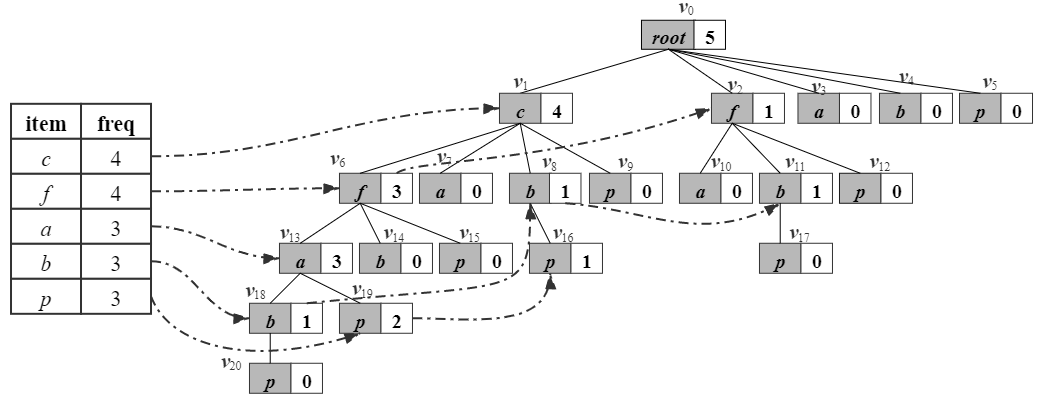
\includegraphics[width=0.5\textwidth]{tree.png}}
\caption{Frequrnt pattern tree(FP-tree).}
\label{fptree}
\end{figure}

\section{Problem Overview }

\subsection{Problem Definition}
In this paper, we look at the privacy preserving frequent itemset mining problem in the local setting and discover $top-k$ frequent itemsets as well as their frequencies while fully consider users' personal privacy. Formally, let $\mathcal{X} = \{x_1,x_2,...,x_d\}$ be a set of items, the length-$|X|$ itemset $X$ is a subset of $\mathcal{X}$, i.e.,$X \subseteq \mathcal{X}$, where $|X|$ denote its cardinality.

In general, there are $n$ users, and each user has a sensitive transaction (or set value), which is a subset of $\mathcal{X}$. The transaction of $i$-th user is $T_i(i \in [1,n])$ and $\mathcal{T} = \langle T_1,T_2,...,T_n \rangle$ denote the whole transaction database. An untrusted data analyst (or aggregator) is aimming to mine $top-k$ most frequent itemsets and their frquencies among all users under LDP. More specifically, we focus on discovering $k$ length-$\alpha$ itemsets with highest frequencies, where $\alpha \geq 2$, while discovering length-1 itemsets (or items) under LDP may take advantage of PSFO protocol (such as SVIM).
%如果将方案中改为 选择top-2k的 length-1集合,去收集任意长度的集合 其效果怎么样

{\color{red}Table \ref{notations} lists the notations used in this paper}

\begin{table}[!t]
\caption{Notations.}
\begin{center}
\begin{tabular}{|c|c|}\hline
  Symbol&Description \\\hline
  $n$ & the number of users \\\hline
  $X$ & the itemset \\\hline
  $|X|$ & the cardinality of itemset $X$ \\\hline
  $\mathbb{G}(X)$ & the guessing frequency of $X$ \\\hline
  $\tilde{\theta}(X)$ & the estimated frequency of $X$ \\\hline
  $\mathcal{T}$ & the transaction database \\\hline
  $T_i$ & the transaction of user $i$ \\\hline
  $\mathcal{X}$ & the item domain \\\hline
  $d$ & the size of item domain, $d = |\mathcal{X}|$ \\\hline
  $\hat{\mathcal{N}}$ & the noisy FP-tree \\\hline

\end{tabular}
\label{notations}
\end{center}
\end{table}

\subsection{The Existing Approache to FIM under LDP}\label{svim and svsm}
Since Qin et al.\cite{a1} first introduce set-valued setting to differential privacy in the local setting for the purpose of discovering heavy hitters as well as their frequencies, it has been a challenge that mining frequent itemsets from all sanitized data. To the best of our konwledge, only SVSM\cite{a2} protocol that implements effectively FIM task in context of LDP. Particularly, it focuses on mining $top-k$ most frequent length-$\alpha$ ($\alpha\geq2$) itemsets while applying SVIM\cite{a2} protocol to obtain the $k$ frequent items (or length-1 itemsets) as initial condition to construct candidate set. Details as follows. 

$Set-Value\ Item\ Mining\ (SVIM)$: SVIM is a PSFO protocol with the same problem setting as LDPMiner\cite{a1}, which focus on discovering the $k$ frequent items with highest frequencies. It has four steps and divide proportionally all users into three mutually disjoint groups $G_1,G_2,G_3$ so that each user is protected by $\epsilon$-LDP.

\textbf{1. Prune the Domain --- $G_1$.} The goal is to identify a candidate set of items so that it can narrow down the domian size into $2k$, which is greatly less than $d$. In this step, each user uses FO to perturb a randomly sampled item from her raw data. Then, the analyst estimates the frequency of each value in the whole domain $\mathcal{X}$ and selects the $2k$ items with highest frequencies as pruned domian $S$. The analyst broadcasts the set $S$ pruned to all users.

\textbf{2. Size Estimation --- $G_2$.} To further estimate the frequency of items in $S$, it is necessary to approximate the distribution of the number of frequent items that users hold due to the technique that padding-and-sampling (PS). Thus, with OLH protocol, the data of each user in this step is the size of the raw data intersected with $S$. After the perturbing finishes, the alalyst estimates the length distribution and computes the $\gamma = 90\%$ length $L$ by  
\begin{equation}
\frac{\sum_{i=1}^{L} \tilde{\theta}(i)}{\sum_{i=1}^{2k} \tilde{\theta}(i)} > \gamma \label{length}
\end{equation}
where $\tilde{\theta}(i)$ denote the estimated number of users' data length is $i$. 

\textbf{3. Frequencies Estimation --- $G_3$.} Once the analyst gets $S$ and $L$, it will use PSFO protocol to precisely estimate the frequencies of the items in small domian $S$. That is, each user first pads his pruned data, which is the raw data intersected with $S$, to length $L$, then applies FO protocol to perturb an item that randomly choose. 

Finally, for each item in $S$, the analyst computes its estimated frequency over all sanitized data. Note that the estimated frequency needs to be multiplied by $L$ to ensure it is unbiased.

\textbf{4. Estimation Update.} Due to $L$ is the 90th percentile length, which may lead to an underestimate. In order to improve the accuracy of the estimations, an update factor $u(L)$ is defined for correcting this under estimation. Practically, in this step, every frequency estimated is multiplied with the update factor $u(L)$.
$$u(L) := \frac{\sum_{i=1}^{2k} \tilde{\theta}(i)}{\sum_{i=1}^{2k} \tilde{\theta}(i) - \sum_{i=L+1}^{2k} \tilde{\theta}(i)(i-L) }$$

Note that step 4 is does not consume the privacy budget because informations are obtained from previous steps and there is no user involved. When all the steps are done, the $k$ items with highest frequencies are selected with high confidence. However, SVIM cannot be used directly ro mine itemsets that has exponential domian. Therefore, Set-Value itemSet Mining (SVSM) is proposed with the core technique named ``Guessing Frequency (GF)'' to construct a pony-sized domian of itemsets.

%Summarily, we summarize it in three phases: Prune the Domain and Frequency Estimation. The fomer identifies a candidate set for items so that it can reduce the domian size into $2k$, which is greatly less than $d$ when $d$ is large; Then, the latter focuses on the frequent items identified to estimate precisely their frquencies in small domain.

$Set-Value\ itemSet\ Mining\ (SVSM)$: As mentioned above, SVSM needs to know the set of $top-k$ frequent items, denoted by $S^{\prime}$. Then, to construct candidate set of itemsets, the guessing frequency of each  exponentially possible itemset that made up of items in $S^{\prime}$ is calculated by \eqref{gf}, and the pony-sized domain set $IS$ is constructed by selecting $2k$ itemsets with highest guessing frequencies.

\begin{Definition}
(GF). Let itemset $X$ is a subset of a set of items $\{{x_1,x_2,...,x_m} \}$, and the support of the item $x_i$ is denoted by $\theta(x_i)$. The guessing frequency (GF) of $X$ is $\mathbb{G}(X)$, defined as follows,\\
\begin{equation}
\mathbb{G}(X) = \prod_{x \in X} \frac{\lambda \times \theta(x)}{\theta_{max}} \label{gf}
\end{equation}
where $\theta_{max}$ is the maximum support of all items, $0 \leq \lambda \leq 1$ is a predifined parameter.

\end{Definition}

When the domain of candidate itemsets is pruned, it may use following steps of SVIM to discover frequent itemsets. Note that every user's sensitive data is the power set of her raw data intersected with $S^{\prime}$.

\textbf{Flaw.} However, it is obvious that there are exponentially more possible itemsets during constructing candidate set. For example, such $k$ items produce $2^{k}$ possible itemsets, leaving considerable computational cost in guessing frequencies. Although it is persuasive that the cardinality of frequent itemset would not be greater than $\log_{2} k$, the computational space $O\left(\sum_{i=2}^{\lfloor \log_{2}k \rfloor} \dbinom{k}{i} \right)$ is not acceptable when $k$ is large.

\section{fpmine: the FP-tree-based Approach}
In this section, we propose a novel FP-tree-based mining approach called $FPmine$ that discovers the $top-k$ most frequent itemsets under LDP with low computational cost as well as high accuracy. The main idea is to constrcut a noisy FP-tree, and then discover itemsets over the tree. In the following, Section \ref{fpmine} overviews the framework of $FPmine$. Section \ref{construct and mine} describes the details of constructing and mining the nosiy FP-tree. Sections \ref{cutdown candidate} and \ref{optimize} further optimize the proposed approach, respectively.

\subsection{FPmine}
\label{fpmine}
As described in Section \ref{svim and svsm}, the existing solutions incur considerable computational cost duo to the exponential growth of candidate itemsets. We observe that the FP-growth algorithm can mines frequent itemsets without a costly candidate generation process, which significally reduce the cost. However, in the local setting, the analyst's inability to access users' raw data makes it difficult to constrcut a noisy FP-tree over sanitized data. Note that if we can decrease the scale of the added noise, then we can efficiently reduce the computational cost as well as achieve better accuracy. Algorithm \ref{alg fpmine} presents the procedure of FPmine.

Specifically, FPmine first constructs a noisy FP-tree in a breadth-first manner for the purpose of storing informations without compromising privacy, and then mines frequent itemsets by pattern fragment growth. Observe that the domain size $d$ of items might be large in practice and only a set (or combination) of frequent items is possible to be a frequent itemset. For instance, there are five transactions in Table \ref{trans table}. While no transaction appears more than once, as items $a,b,c,f$ and $p$ are identified as frequent, the possible frequent itemset must be a set of frequent items, such as $\{c,f\},\{a,b,c\}$ and $\{f,p\}$. Therefore, it is necessary and meaningful to identify the $k$ frequent items, which may significantly narrow the candidate itemsets. 

In short, FPmine works as follows: First, a set of frequent items are identified with SVIM protocol. Second, OLH is used to approximate the maximum number of frequent items that user holds. Third, it constructs a noisy FP-tree in a breadth-first manner, and then mines the tree for frequent itemsets.

\begin{algorithm}[htbp]
  \caption{FPmine($\mathcal{T},\mathcal{X},k,\epsilon$)}
  \label{alg fpmine}
  \begin{algorithmic}[1]
  \REQUIRE transactional database $\mathcal{T}$, set of items $\mathcal{X}$, top $k$, privacy budget $\epsilon$
  \ENSURE a set of frequent itemsets $\tilde{\mathcal{P}}$

  \STATE Randomly divide $\mathcal{T}$ into three groups $G_1,G_2,G_3$; \label{fpmine group}
  \STATE Collect the items set $S^{\prime} \gets SVIM(G_1,k,\epsilon)$; \label{fpmine items}
  
%80百分位长度
  \STATE Each user in group $G_2$ perturbs the number of frequent items he holds to analyst with OLH$({\epsilon})$;\label{fpmine length first}
  \STATE {\color{red}$\mathcal{L} \gets \frac{3\cdot \sqrt{|G_2|}}{\epsilon}$};\label{fpmine T}
  \FOR{length $l=1$ to $k$}  
    \STATE Compute the frequency $\tilde{\theta}(l)$;
    %\STATE Apply OLH protocol to collect information from users of group $\mathcal{T}_2$ to estimate $\tilde{\theta}(l)$ using privacy budget $\epsilon$;
    \IF{{\color{red}$\tilde{\theta}(l) < \mathcal{L}$}}
      \STATE $\tilde{\theta}(l) \gets 0$;
    \ENDIF
  \ENDFOR
  \STATE Compute $L_{m}$ by \eqref{length} where $\gamma=80\%$;\label{fpmine Lm}

  \STATE $\hat{\mathcal{N}} \gets ConstructNoisyTree(G_3,S^{\prime},L_m,\epsilon)$;
  \STATE Mine the $k$ itemsets $\tilde{\mathcal{P}}$ with highest frequencies; \label{fpmine mine}
  \RETURN $\tilde{\mathcal{P}}$
  \end{algorithmic}
\end{algorithm}

As shown in algorithm \ref{alg fpmine}, given the privacy budget $\epsilon$, similar to SVSM is that we divide all users into three groups $G_1,G_2,G_3$ to participate in each step (line \ref{fpmine group}), which provides $\epsilon$-LDP for each user. That is, the first step is aiming to identify the set $S^{\prime}$ of $k$ frequent items from users in $G_1$ with SVIM protocol (line \ref{fpmine items}). And then the second is to approximate the maximum number of frequent items that user holds (line \ref{fpmine length first}-\ref{fpmine Lm}). In this step, the 80th percentile length $L_m$ is calculate by \eqref{length} while the differences are that we set $\gamma=80\%$ (line \ref{fpmine Lm}) and initialize a threshold {\color{red}$\mathcal{L}$} (line \ref{fpmine T}) based on Lemma \ref{olh error} to filter the estimates. Finally, on receiving $S^{\prime}$ and $L_m$, the noisy FP-tree {\color{red}$\hat{\mathcal{N}}$} is constrcuted by $ConstructNoisyTree$ (Algorithm \ref{alg ConstructNoisyTree} in Section \ref{construct and mine}), and then the analyst can discover accurate itemsets by pattern fragment growth (line \ref{fpmine mine}), which follows the procedure of the FP-growth except accumulating frequencies of conditional patter bases as explained in Section \ref{construct and mine}. 

Note that FPmine divides all users into three groups, groip $G_1$ for frequent items, group $G_2$ for maximum length and $G_3$ for noisy FP-tree. Each group provides $\epsilon$-LDP for each user, thus the whole process satisfies $\epsilon$-LDP.

\begin{lemma}
Algorithm \ref{alg fpmine} satisfies $\epsilon$-LDP.
\end{lemma}

%\begin{proof}
%Note that FPmine divides all users into three groups, group $G_1$ for frequent items, group $G_2$ for maximum length and $G_3$ for noisy FP-tree. Each group provides $\epsilon$-LDP for each user, thus the whole process satisfies $\epsilon$-LDP.
%\end{proof}

\begin{lemma}\label{olh error}
For any estimated frequency $\tilde{\theta}$ obtained by OLH and $\theta$ is the exact frequency. With at least $1-\beta$ probability, we have:
$$|\tilde{\theta} - \theta | = O \left(\frac{\sqrt{n\ln{(1/\beta)}}}{\epsilon} \right)$$
where $n$ is the number of users that participated.
\end{lemma}

\subsection{Constructing and mining the noisy FP-tree}
\label{construct and mine}
In the local setting, the main challenge of constructing a noisy FP-tree is that the analyst has no right to access users' raw data, and that leads to introduce considerable noise when the tree is constructed. In \cite{fp}, the non-privacy FP-tree is constructed by scanning unconcealed transactions and {\color{red}updating nodes with frequent items that user holds in a depth-first manner}. We observe that it enables to construct the FP-tree in a breadth-first manner if the final count of each node at same level is known in advance. Inspired by this, we propose a breadth-first approach {\color{red}called $ConstructNoisyTree$} to costruct a noisy FP-tree layer by layer. Specifically, let $L_m$ is the maximum length, and $x_1 \succ x_2 \succ \cdots  \succ x_k$ is the ordered sequence of $k$ frequent items, denoted by $S^{\prime}$, where $x_i \succ x_{i+1}$ means that $x_i$ is more frequent than $x_{i+1}$ and $x_i$ comes before $x_{i+1}$. The {\color{red} $ConstructNoisyTree$} has two phase:

%$S^{\prime} = \left [ x^1 : \tilde{\theta}(x^1),  x^2 : \tilde{\theta}(x^2),...,x^k : \tilde{\theta}(x^k) \right ]$ denote the sorted sequence of $k$ frequent items as well as their frequencies, where $\tilde{\theta}(x^i)$ denote the frequency of a frequent item $x^i$ and for any $i>j$, it has $\tilde{\theta}(x^i) \geq \tilde{\theta}(x^j)$. For convenience, we abuse notation and use $S^{\prime}$ to denote the set of frequent items that identified.

% 或许可以将两个表并排放
\begin{table}[tb]
\caption{{\color{red}Preprocessed transactional data.}}
\label{preprocessed trans}
\centering
\begin{tabular}{|c|l|}\hline
  TID&List of items \\\hline
  T01&$c,f,a,p$ \\\hline
  T02&$c,f,a,b$ \\\hline
  T03&$f,b$ \\\hline
  T04&$c,b,p$ \\\hline
  T05&$c,f,a,p$ \\\hline
\end{tabular}
\end{table}

%不需要介绍先用SVIM获得频繁单项,可以当作BSL就是之后的步骤去介绍
\textbf{Phase \uppercase\expandafter{\romannumeral1} Preprocessing.} All participating users first delete infrequent items in their transactions and then rearrange the rest in order of $S^{\prime}$. For example, while the frequent items in Table \ref{trans table} is sorted to $c\succ f\succ a\succ b\succ p$, then the preprocessed transactional data is shown in Table \ref{preprocessed trans}.

Additionally, after the preprocessing step finishes, there are many infrequent items discarded, which significantly cuts down the size of candidate sets and achieves good performance because of the Apriori property\cite{apr}: {\color{red} $only\ if\ the\ length-\alpha\ itemset\ is\ frequent\ are\ its\ length-(\alpha +1)\ supersets\ likely\ to\ be\ frequent.$}

\textbf{Phase \uppercase\expandafter{\romannumeral2} Constructing the FP-tree} In contrast to FP-growth, we propose a breadth-first approach to construct a noisy FP-tree layer by layer in the local setting. Details described in Algorithm \ref{alg ConstructNoisyTree}. 

Note that we omit the mining procedure duo to the fact that it is similar to the original algorithm and remark on the differences.

\begin{itemize}
\item A node $v$ in the FP-tree has two fields: $v.item$ and $v.count$, where denote the indicated item of node $v$ and the number of its prefix $pre(v)$ in transactions respectively.
\item The informations of the $S^{\prime}$ and $L_m$ are obtained in a way that satisfies the $\epsilon$-LDP. The formar is used to arrange users' frequent items and the latter marks the end of constructing the FP-tree. This ensures that the noisy FP-tree does not depend on any specific transaction.
\item We construct the FP-tree in a breadth-first manner, which is unlike to the original algorithm, that is, the information is collected for updating the tree nodes layer by layer. Notablely, the input value of each user in $l$-th level is either an element of the candidate prefix set $C_l$ or the dummy value $\dagger$. Therefore, we only use the existing FO protocol (e.g. OLH) with the finite domain $C_l \cup \dagger$ to collect information at each level.
\item We randomly divide users into $L_m$ equal-sized groups and users in each group use the full privacy budget $\epsilon$. It turns out that the overall process achieves better accuracy and satisfies $\epsilon$-LDP as well (\cite{a8,privtrie}).
\item {\color{red} Let $X$ denote a discovered itemset and its estimated frequency $\tilde {\theta}(X)$ is unbiased. Note that $\tilde {\theta}(X)$ is obtained from $m$ conditional patter bases $B_1,B_2,...,B_m$. Unlike the original algorithm to add directly, the final $\tilde {\theta}(X)$ is calculated in a way that minimize its variance as in Theorem \ref{minimized noisy count}. 
%$Var(\tilde {\theta}(X)) = \mathbb{E}\left[ \big(\tilde{\theta}(X) - \theta (X) \big)^2 \right]$.


%we calculate the weighted value $\tilde {\theta}(X) = \sum_{i=1}^{m} \omega_i \tilde{\theta}(B_i)$ as its frequency, where $\sum_{i=1}^{m}\omega_i = m$. Theorem \ref{x} shows the variance is minimized by setting $\omega_i = m \cdot \frac{1/r_i }{\sum_{j=1}^{m} \frac{1}{r_j} }$



%To correct  then we  the weighted value $\tilde {\theta}(X) = \sum_{i=1}^{m} \omega_i \tilde{\theta}(B_i)$ is calculated as its frequency, where $\sum_{i=1}^{m}\omega_i = m$.\\

% by setting $\omega_i = m \cdot \frac{1/r_i }{\sum_{j=1}^{m} \frac{1}{r_j} }$, where $\sum_{i=1}^{m}\omega_i = m$ and $r_i$ is the variance of the estimated counts of $B_i$ . The proof is presented in Theorem  \\
-----!!Notice whether it's different from a linear combination!!-----}
%这里是需要 $X= B_1+ ... + B_m$  而不是线性组合使系数为1.

%the existing FO protocol (e.g. OLH) is used to collect information for updating the tree nodes 
\end{itemize}

\begin{theorem}\label{minimized noisy count}
Given $m$ noisy counts $\tilde{\theta}(b_1),\tilde{\theta}(b_2),...,\tilde{\theta}(b_m)$ with variances of $r_1,r_2,...,r_m$. The variance of $X = \sum_{i=1}^{m}\omega_i\tilde{\theta}(b_i)$ with constrain $\sum_{i=1}^{m}\omega_i = m$ is minimized by setting $\omega_i = m \cdot \frac{r_i^{-1} }{\sum_{j=1}^{m} r_j^{-1}}$.
\end{theorem}

\begin{proof}
Obviously, with $\sum_{i=1}^{m}\omega_i = m$, finding the minimized variance of $X = \sum_{i=1}^{m}\omega_i\tilde{\theta}(b_i)$ is equivalent to solve
\begin{equation}
\min{\sum_{i=1}^{m}\omega_i r_i , s.t. \sum_{i=1}^{m}\omega_i = m } \label{weigh mine}
\end{equation}

Then, we have the Lagrangian function
$$\mathcal{L} = \sum_{i=1}^{m}\omega_i r_i + \lambda(m - \sum_{i=1}^{m}\omega_i)$$

Let $\frac{\partial {\mathcal{L}}}{ \partial{\omega_i}} = 2r_i \omega_i - B$ be zero, we have $\omega_i = \frac{\lambda}{2r_i}$. And according to the condition $\sum_{i=1}^{m}\omega_i = m$, we get the constant $\lambda = \frac{2m}{\sum_{i=1}^{m} r_i^{-1}}$.

Finally, we have the optimal solution is $\omega_i = m \cdot \frac{r_i^{-1} }{\sum_{j=1}^{m} r_j^{-1}}$.

\end{proof}



\begin{algorithm}[htbp]
  \caption{ConstructNoisyTree($G_3,S^{\prime},L_m,\epsilon$)}
  \label{alg ConstructNoisyTree}
  \begin{algorithmic}[1]
  \STATE Randomly and evenly divide users into $L_m$ groups $g_1,g_2,...,g_{L_m}$ with $n_g = \lfloor \frac{n}{L_m} \rfloor$ users each;
  \STATE Initialize the tree $\hat{\mathcal{N}}$ with a root node $v_r$; \label{ConstructNoisyTree tree}
  \STATE Initialize the count of $v_r$ is $n_g$ and mark it as valid;\label{ConstructNoisyTree root}

  \STATE Preprocess transactions of all participating users;

  \FOR{$l=1$ to $L_m$}
    \WHILE{there exists a valid node $v$ and $v.count > 0$}
      \STATE Initialize a candidate prefix set $C_l = \emptyset$;
      \STATE Mark $v$ as unvalid;
      \FOR{each item $x \in S^{\prime}$ and $v.item \succ x.item $} \label{ConstructNoisyTree add child}
        \STATE Add a child $v_c$ of $v$ with item is $x$ and count is 0;\label{ConstructNoisyTree child}
        \STATE Mark $v_c$ as valid and compute its prefix $pre(v_c)$;\label{ConstructNoisyTree child prefix}
        \STATE $C_l \gets C_l \cup pre(v_c)$;\label{ConstructNoisyTree child prefix set}
%Add the $pre(v_c)$ to candidate prefix set $C_l$; \label{ConstructNoisyTree child prefix set}
      \ENDFOR
    \ENDWHILE
 
    \IF{$C_l$ is $\emptyset$}
    \STATE Break;
    \ENDIF
    
    %\STATE $C^{\prime}_{l}=NarrowCandidate(S^{\prime},C_l,\xi)$; \label{ConstructNoisyTree narrow}

    \FOR{each users in group $g_l$} \label{ConstructNoisyTree estimate}
    \STATE Perturbe his first $l$ items with OLH protocol for collecting and updating an estimation count $\tilde{\theta}(v)$ of each node $v$, whose prefix is in $C_{l}$;
    \ENDFOR

    \STATE Update nodes at $l$-th level of $\hat{\mathcal{N}}$; \label{ConstructNoisyTree update}
  \ENDFOR

  \RETURN The noisy tree $\hat{\mathcal{N}}$.
  
  \end{algorithmic}
\end{algorithm}

%举例介绍图中模式树的建立过程。
For example, lets consider the processed transactions in Table \ref{preprocessed trans}, where the frequnet items and their supports is denoted by $S^{\prime} = \left[c:4 , f:4 , a:3 , b:3, p:3  \right]$ (for simplicity, we use the real support below). Then, the root node $v_0$ is initialized firstly as the 0-th level of the tree $\hat{\mathcal{N}}$ (line \ref{ConstructNoisyTree tree}-\ref{ConstructNoisyTree root}) and the constructing process is as follows.

At the 1-st level, the children $v_1,v_2,v_3,v_4,v_5$ of $v_0$ are added to form the candidate node at the 1-st level of the tree, which initialized each count is zero (line \ref{ConstructNoisyTree child}). And then according to the candidate prefix set $C_1 = \left\{ (c),(f),(a),(b),(p) \right\}$, their estimated informations are collected for the purpose of updating nodes' counts (line \ref{ConstructNoisyTree estimate}-\ref{ConstructNoisyTree update}), that is, the counts of $v_1,v_2$ are updated to 4 and 1 while $v_3,v_4,v_5$ are pruned according to the collected information $\left\{ (c,4),(f,1),(a,0),(b,0),(p,0) \right\}$. After the 1-st level are updated, the candidate set $C_2 = \left\{ (c,f),(c,a),(c,b),(c,p),(f,a),(f,b),(f,p) \right\}$ at the 2-nd level is constructed. Then it can update the tree nodes in the same way while the transaction of each user is the first two items in his pre-processed data (e.g. the input value of first user  is $(c,f)$). $ConstructNoisyTree$ continues to the next iteration until the tree reaches its maximum level $L_m$ or there are no node is valid. The final FP-tree is constructed as show in Fig. \ref{fptree}.

\begin{lemma}
Algorithm \ref{alg ConstructNoisyTree} satisfies $\epsilon$-LDP.
\end{lemma}

\begin{proof}
proof Algorithm satisfies LDP.
\end{proof}

\begin{lemma}
For any node $v$ in the tree, let $\tilde{\theta}(v)$ denote its estiamted count obtained by the algorithm \ref{alg ConstructNoisyTree} and $\theta (v)$ denote the ground truth. With at least $1-\beta$ probability, we have:
$$|\tilde{\theta}(v) - \theta(v) | = O \left(\frac{L_m...}{\epsilon} \right)$$
\end{lemma}

\subsection{Cutting down the cadidate prefix set}
\label{cutdown candidate}
We observer that the biggest limitation of ConstructNoisyTree is that the size of candidate prefix set $C_l$ constructed during $l$-th iteration is indisciplinable and large. Deu to $C_l$ is the prefixes domian of OLH to gather estimations, the large size affects not noly accuracy but also computational cost. Observe that the size of $C_l$ is linearly related to nodes reserved in the upper $(l-1)$-th level. That is, the fewer nodes are reserved in $(l-1)$-th level, the fewer children are generated in $l$-th level, which makes up small $C_l$. However, it is inefficient since reserving fewer nodes may result in information loss and underestimation.  

In view of this, {\color{red}we set a threshold to remove as many invalid nodes as possible while retain effective estimations. Formally, let $v$ is a node of the tree while $v.count$ is initialized to zero before estimation. Once we obtain an estimated count $\tilde{\theta}(v)$ of its prefix $pre(v)$, the threshold is used to determine if it is valid. Specifically, $v$ is valid when $\tilde{\theta}(v) > \mathcal{L}^{\prime}$ and invaild otherwise. Finally, we update $v.count=\tilde{\theta}(v)$ when $v$ is valid and $v.count=0$ when it is invalid. It is noted that the larger threshold, the fewer invalid estimations, but more valid values may be lost. In this paper, we set threshold $\mathcal{L} = \frac{3\cdot \sqrt{|G_2|}}{\epsilon}$, which is the maximum error boundary of OLH.}

Sequentially, it is obvious that there are many redundant prefixes in $C_l$. For example, at the 3-rd level of the tree in Fig. \ref{fptree}, the initial set $C_3$ is made up of prefixes of $v_6,v_7,v_8,v_9,v_{10},v_{11},v_{12}$. However, as the information is collected, four invalid nodes $v_7,v_9,v_{10},v_{12}$ are removed. Recall from users' transanctions that there are no prefixes for these nodes. Therefore, if we can remove beforehand as many of these as possible, then the size will be significantly narrowed.

Similar to SVSM\cite{a2} is to limit the candidate set to a fixed size. We propose $CutdownCandidate$ (Algorithm \ref{alg:cutdown candidate}) to further narrow the set $C_l$ down to fixed size $\xi \cdot k \ll |C_l|$, where $\xi$ is a predefined adiustable parameter. Specifically, when the size is greater than $\xi \cdot k$, we first guess each candidate prefix in $C_l$. And then select the $top-\xi k$ prefixes with highest guessing frequencies to construct a pony-size set $C^{\prime}_{l}$. Note that each prefix in $C_l$ has the same cardinality and we just need to get their relative order. Therefore, we use the simplified guessing frequency $\mathbb{G}^{\prime}(P)$ of prefix $P \in C_l$ to construct $C^{\prime}_{l}$,
\begin{equation}
\mathbb{G}^{\prime}(P)=\prod_{x \in P} \tilde{\theta}(x) \label{simply gf}
\end{equation}
where $\tilde{\theta}(x)$ is the frequency in $S^{\prime}$ of item $x$.

%we guess the frequency of candidate itemsets in $C_i$, and then select the $\xi \cdot k$ itemsets with highest guessing frequency. Details in algorithm \ref{alg:narrow candidate}.

\begin{algorithm}[]
\caption{CutdownCandidate($S^{\prime},C_l,\xi$)}
\label{alg:cutdown candidate}
\begin{algorithmic}[1]

\STATE Initialize $d_c \gets C_l$;
\STATE Initialize $C^{\prime}_{i} = \emptyset$;
\IF{$d_c > \xi k$}
  %\STATE Initialize $C^{\prime}_{l} = \emptyset$;
  \FOR{each candidate prefix $P \in C_l$}
    \STATE Guess the frequency $\mathbb{G}(P)=\prod_{x \in P} \tilde{\theta}(x)$ of $P$;        
  \ENDFOR
  \STATE Construct $C^{\prime}_{l}$ by selecting the $\xi k$ prefixes in $C_l$ with highest guessing frequencies;

\ELSE
  \STATE $C^{\prime}_{l} \gets C_l$

\ENDIF 

\RETURN $C^{\prime}_{l}$
\end{algorithmic}
\end{algorithm}

%The other way to reduce the size is to limit it to a fixed size.


\subsection{Imposing consistency and weighted combination}
\label{optimize}
\textbf{Consistency.} Without loss of generality, let $\tilde{\theta}(v)$ denote the noisy count of a node $v$ in the noisy FPtree $\hat{\mathcal{N}}$ that constructed, and $\theta(v)$ is the ground truth. For each node $v$, we have the following constraints:
\begin{itemize}
\item The noisy count $\tilde{\theta}(v)$ is unbiased, and its expectation satisfies $\mathbb{E}[\tilde{\theta}(v)] = \mathbb{E}[\theta(v)]$.
\item If $v$ has a set $S_c$ of children, then\\
$$\mathbb{E}[\tilde{\theta}(v)] \geq \sum_{v_c \in S_c} \mathbb{E}[\tilde{\theta}(v_c)]$$
\end{itemize} 


{\color{red}And the optimal sulotion to find the minimum $L_2$ distance between the noisy tree $\hat{\mathcal{N}}$ and consistency tree $\bar{\mathcal{N}}$ while satisfies constraints is presents in \cite{a5}.}

\textbf{Weighted.} In order to achieve better accuracy, we propose the weighted method, which satisfies post-processing property. Specifically, we weight the results discovered over the tree with guessing frequencies, and then publish the $top-k$ most frequent itemsets. Let $\tilde{P}$ denote the set of itemsets mined from the noisy tree. And for each itemset $X$ in $\tilde{P}$, we have its weighted frequency $\Omega (X) = \omega \cdot \tilde{\theta}(X) + (1-\omega)\cdot \mathbb{G}(X)$, where $\omega \in [0,1]$ is the weighted parameter and $ \tilde{\theta}(X)$ denote the estimated frequency.

%\begin{equation}
%\Omega (X) = \omega \cdot \tilde{\theta}(X) + (1-\omega)\cdot \mathbb{G}(X) \label{weighted frequency}
%\end{equation}

Then, the final $k$ itemsets is obtained by selecting the $k$ itemsets in $\tilde{P}$ with highest weighted frequency.

%\subsection{The weighted combination}

%\subsection{FPmine: the optimal approach}
%We obserbe that the BSmine approach has many flaws that limit its application: (1) the size of candidate prefix set in each iteration affects the accuracy of the FO protocol.

%\section{FPmine: the Optimal Approach}

\section{Experiments}
\subsection{Setup}
\textbf{Metrics}
\begin{itemize}
\item NCR
\item MSE
\end{itemize}

\textbf{Datasets.}
\begin{itemize}
\item Synthetic datasets. {\color{red} generate one or two synthetic datasets following some( normal or Laplace) distributions}
\item Kosarak.
\item POS.
\end{itemize}

\textbf{Settings}



\begin{thebibliography}{00}
\bibitem{MITreview} MIT Technology Review. https://www.technologyreview.com/10-breakthrough-technologies/2020.
\bibitem{a1} Qin, Zhan, et al. "Heavy Hitter Estimation over Set-Valued Data with Local Differential Privacy." computer and communications security (2016): 192-203.
\bibitem{a2} Wang, Tianhao, Ninghui Li, and Somesh Jha. "Locally Differentially Private Frequent Itemset Mining." ieee symposium on security and privacy (2018): 127-143.
\bibitem{a3} Bhaskar, Raghav, et al. "Discovering frequent patterns in sensitive data." knowledge discovery and data mining (2010): 503-512.
\bibitem{a4} Li, Ninghui, et al. "PrivBasis: frequent itemset mining with differential privacy." very large data bases (2012): 1340-1351.
\bibitem{a5} Lee, Jaewoo, and Chris Clifton. "Top-k frequent itemsets via differentially private FP-trees." knowledge discovery and data mining (2014): 931-940.
\bibitem{a6} Zeng, Chen, Jeffrey F. Naughton, and Jinyi Cai. "On differentially private frequent itemset mining." very large data bases (2012): 25-36.
\bibitem{a7} C. Dwork. Differential privacy. In ICALP, pages 1–12, 2006.
\bibitem{fp} Han J, Pei J, Yin Y, et al. Mining frequent patterns without candidate generation[C]. international conference on management of data, 2000, 29(2): 1-12.
\bibitem{apriori} Agrawal R, Imielinski T, Swami A N, et al. Mining association rules between sets of items in large databases[C]. international conference on management of data, 1993, 22(2): 207-216.
\bibitem{apr} Agrawal R, Srikant R. Fast Algorithms for Mining Association Rules in Large Databases[C]. very large data bases, 1994: 487-499.
\bibitem{a8} Wang T, Blocki J, Li N, et al. Locally Differentially Private Protocols for Frequency Estimation[C]. usenix security symposium, 2017: 729-745.
\bibitem{a9} F. D. McSherry. Privacy integrated queries: an extensible platform for privacy-preserving data
analysis. In SIGMOD, pages 19–30, 2009.
\bibitem{eclat} Zaki M J. Scalable algorithms for association mining[J]. IEEE Transactions on Knowledge and Data Engineering, 2000, 12(3): 372-390.
\bibitem{post-processing} C. Dwork, F. McSherry, K. Nissim, and A. Smith, “Calibrating noise to sensitivity in private data analysis,” in Theory of Cryptography Conference. Springer, 2006, pp. 265–284.
\bibitem{rr} S. L. Warner. Randomized response: A survey technique for eliminating evasive answer bias. Journal of the American Statistical Association, 60(309):63–69, 1965.
\bibitem{rappor} U. Erlingsson, V. Pihur, and A. Korolova. Rappor: Randomized aggregatable privacy-preserving ordinal response. In CCS, pages 1054–1067. ACM, 2014.
\bibitem{privtrie} Wang N, Xiao X, Yang Y, et al. PrivTrie: Effective Frequent Term Discovery under Local Differential Privacy[C]. international conference on data engineering, 2018: 821-832.


\bibitem{privkv} Q. Ye, H. Hu, X. Meng and H. Zheng, "PrivKV: Key-Value Data Collection with Local Differential Privacy," 2019 IEEE Symposium on Security and Privacy (SP), San Francisco, CA, USA, 2019, pp. 317-331, doi: 10.1109/SP.2019.00018.
\bibitem{privsuper} N. Wang, X. Xiao, Y. Yang, Z. Zhang, Y. Gu, and G. Yu, “Privsuper:
A superset-first approach to frequent itemset mining under differential privacy,” in ICDE. IEEE, 2017.
\bibitem{apple} J. Tang, A. Korolova, X. Bai, X. Wang, and X. Wang. Privacy loss in
apple’s implementation of differential privacy on macos 10.12. arXiv preprint 1709.02753, 2017.
\bibitem{privacyatscal} G. Cormode, S. Jha, T. Kulkarni, N. Li, D. Srivastava, and T. Wang.
Privacy at scale: Local differential privacy in practice. In SIGMOD, pages 1655–1658. ACM, 2018.
\bibitem{microsoft} B. Ding, J. Kulkarni, and S. Yekhanin. Collecting telemetry data privately. In NIPS, pages 3574–3583, 2017.
\bibitem{apple new words} A. G. Thakurta, A. H. Vyrros, U. S. Vaishampayan, G. Kapoor, J. Freudiger, V. R.
Sridhar, and D. Davidson. Learning new words, Mar. 14 2017. US Patent 9,594,741.
\bibitem{b1} Wang N, Xiao X, Yang Y, et al. Collecting and analyzing multidimensional data with local differential privacy[C]//2019 IEEE 35th International Conference on Data Engineering (ICDE). IEEE, 2019: 638-649.
\bibitem{b2} Yang J, Cheng X, Su S, et al. Collecting Preference Rankings Under Local Differential Privacy[C]//2019 IEEE 35th International Conference on Data Engineering (ICDE). IEEE, 2019: 1598-1601.
\bibitem{b3} Jia J, Gong N Z. Calibrate: Frequency estimation and heavy hitter identification with local differential privacy via incorporating prior knowledge[C]//IEEE INFOCOM 2019-IEEE Conference on Computer Communications. IEEE, 2019: 2008-2016.
\bibitem{b4} Wang D, Xu J. On sparse linear regression in the local differential privacy model[C]//International Conference on Machine Learning. 2019: 6628-6637.
\bibitem{b5} Holohan N, Leith D J, Mason O. Optimal differentially private mechanisms for randomised response[J]. IEEE Transactions on Information Forensics and Security, 2017, 12(11): 2726-2735.


\end{thebibliography}
\vspace{12pt}
\color{red}
IEEE conference templates contain guidance text for composing and formatting conference papers. Please ensure that all template text is removed from your conference paper prior to submission to the conference. Failure to remove the template text from your paper may result in your paper not being published.

\end{document}
